\documentclass{beamer}
\usepackage{graphicx}
\usepackage{tikz}
\usetikzlibrary{shapes,arrows}
\usepackage{tikz}
%\usecolortheme{seahorse}
  \setbeamertemplate{footline}[page number]
\usepackage{multirow}
\setbeamertemplate{navigation symbols}{}
\setbeamertemplate{frametitle}[default][center]
\setbeamerfont{frametitle}{shape=\scshape}
\usepackage{color}

\usepackage{csquotes}

\usepackage{xcolor}

\usepackage[flushleft]{threeparttable}

{\title{\textsc{Econ 352 - Business Cycle Models with Flexible Prices and Wages} \\ \tiny (See Williamson Ch. 13)}
\author{Trevor S. Gallen}
\date{}
\begin{document}
\renewcommand*{\inserttotalframenumber}{\pageref{lastframe}}


\setbeamertemplate{caption}{\raggedright\insertcaption\par}

\begin{frame}
\titlepage
\end{frame}

\begin{frame}
\frametitle[alignment=center]{Introduction}
\begin{itemize}
\item We have an intertemporal model with money
\bigskip
\item We now want to see how it might explain the business cycle
\bigskip
\item We'll see some successes, but some possible failures as well
\bigskip
\item This will motivate adding some frictions
\end{itemize}
\end{frame}

\begin{frame}
\frametitle[alignment=center]{Real Shocks}
\begin{itemize}
\item Can fluctuations in U.S. economic activity be reconciled with real shocks?
\smallskip
\item Imagine that TFP, $z$ is fluctuating around
\bigskip
\item As we saw (and will see) $z$ is persistent, so $z$ and $z'$ are correlated
\bigskip
\item How does the economy react when $z$ and $z'$ increase?  
\bigskip
\item $z,z'\uparrow$, $MPL\uparrow$, so $N^d_1\uparrow$ and $N^d_2\uparrow$, and $Y_1^s\uparrow$ and $Y_2^s\uparrow$
\item Because $MPK\uparrow$\ and lifetime income $\uparrow$, $Y^d_1$ and $Y^d_2\uparrow$
\item We think $r$ falls, as investment highly responsive due to income differences over time
\item Money demand rises ($r$ falls, $Y$ rises) so $P$ \emph{falls}
\end{itemize}
\end{frame}


\begin{frame}
\frametitle[alignment=center]{``Productivity" Shocks are Correlated with GDP}
\begin{figure}
\centering
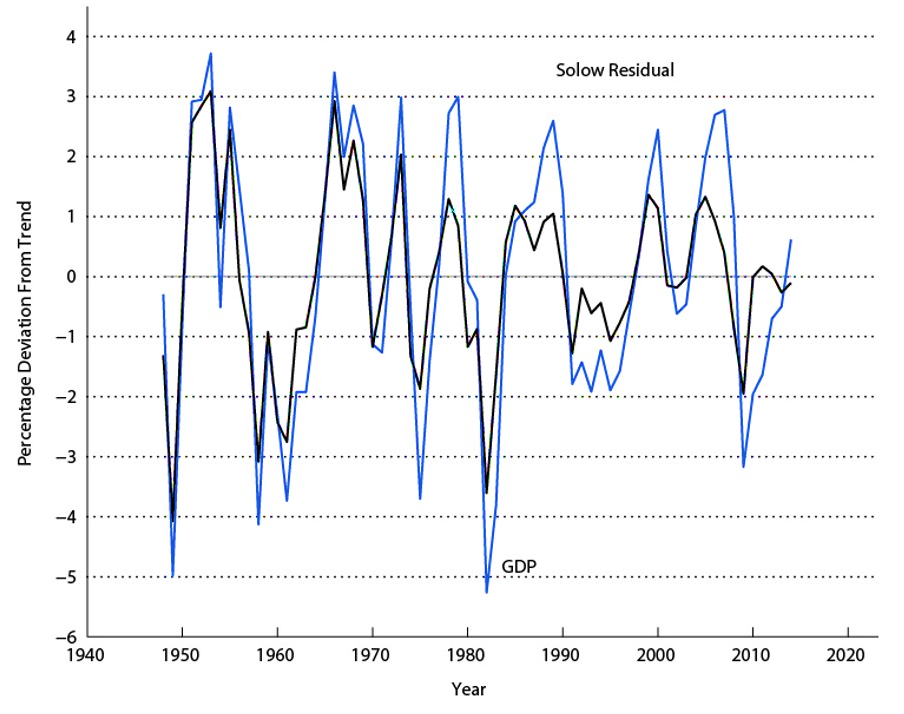
\includegraphics[scale=0.65]{Figures/W_Fig_13pt1.png}
\end{figure}
\end{frame}


\begin{frame}
\frametitle[alignment=center]{Summary of Model Effects}
\begin{figure}
\centering
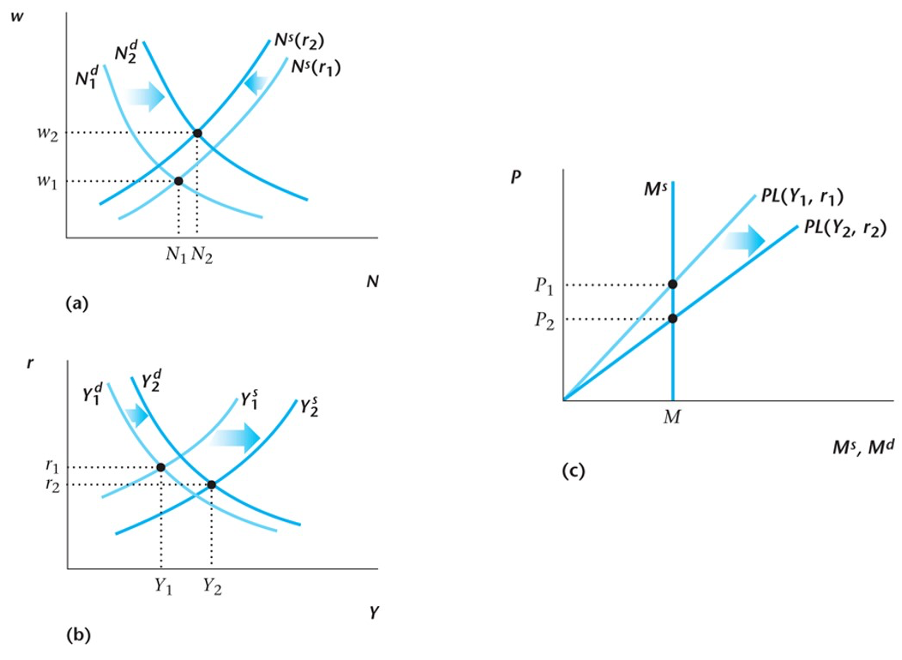
\includegraphics[scale=0.65]{Figures/W_Fig_13pt2.png}
\end{figure}
\end{frame}


\begin{frame}
\frametitle[alignment=center]{Effect on Average Productivity}
\begin{figure}
\centering
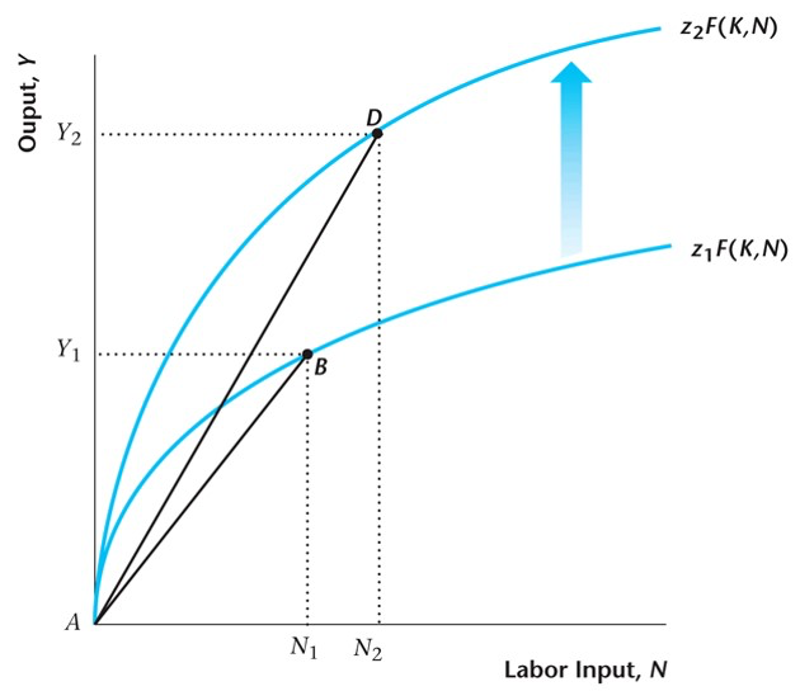
\includegraphics[scale=0.65]{Figures/W_Fig_13pt3.png}
\end{figure}
\end{frame}


\begin{frame}
\frametitle[alignment=center]{Summary of the RBC Model Predictions}
\begin{table}
\centering
\begin{tabular}{lcc}
\hline\hline
Variable & Data & Model \\
\hline
Consumption & Procyclical & Procylical \\
Investment & Procyclical & Procylical \\
Employment & Procyclical & Procylical \\
Real Wage & Procyclical & Procylical \\
Average Labor Productivity & Procyclical & Procylical \\
Price level & ??? & countercyclical(?) \\
\hline\hline
\end{tabular}
\end{table}
RBC model does a pretty good job, generally!  One reason why it has stuck around as the kernel of most other Macro models
\end{frame}

\begin{frame}
\frametitle[alignment=center]{Thinking a little more about money}
\begin{itemize}
\item In our RBC model, the price level is countercyclical (if monetary policy passive)
\bigskip
\item But, empirically (and historically):
\begin{itemize}
\item Nominal money supply is procyclical (higher GDP, more money printed)
\bigskip
\item Nominal money supply leads GDP
\end{itemize}
\item How can we reconcile with the model?
\bigskip
\item We assumed monetary policy is passive (and exogenous)--but if money is endogenous perhaps not
\end{itemize}
\end{frame}

\begin{frame}
\frametitle[alignment=center]{Reconciling Prices and the RBC Model}
\begin{itemize}
\item Let's say that fluctuations are actually caused by TFP shocks, $z$
\bigskip
\item Banking sector activity higher ($pH$ higher in limited commitment, investment higher, etc.)
\bigskip
\item So banking deposits $M1$, $M2$ rise
\bigskip
\item So, with an increase in TFP, and decrease in the interest rate, causes prices to fall
\bigskip
\item But if $P$ is held constant, then central bank should increase $M$ 
\bigskip
\item This is consistent with the fact that $M$ is procyclical
\bigskip
\item But still an issue!  $M$ leads $Y$, so isn't it causal?
\end{itemize}
\end{frame}

\begin{frame}
\frametitle[alignment=center]{Effect on Average Productivity}
\begin{figure}
\centering
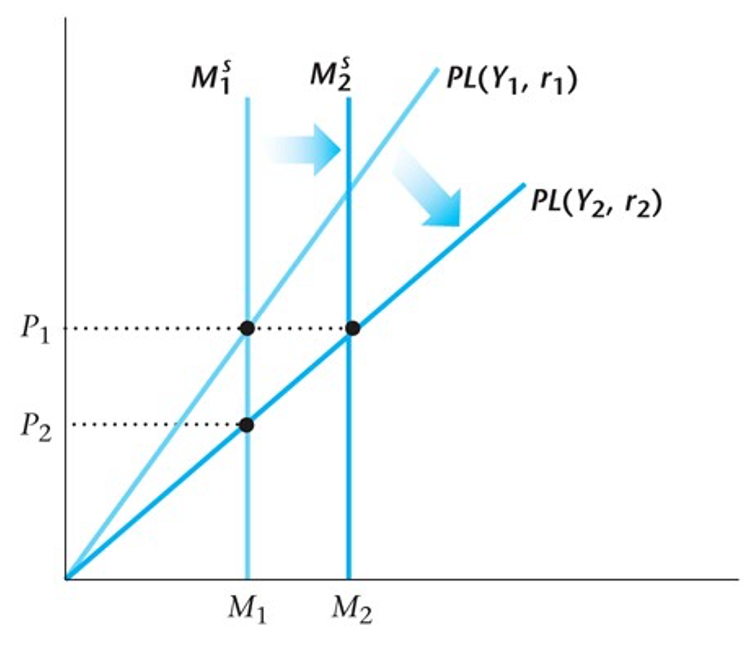
\includegraphics[scale=0.65]{Figures/W_Fig_13pt4.png}
\end{figure}
\end{frame}


\begin{frame}
\frametitle[alignment=center]{Issue: $M$ leads $Y$}
\begin{itemize}
\item If $M$ leads $Y$, it's a stronger case that it causes $Y$
\bigskip
\item But not always, particularly with humans: hit the brakes before the light turns red, but hitting the brakes doesn't cause the light to turn red!
\bigskip
\item But if $z$ affects bank activity, which affects $M1$, $M2$
\bigskip
\item Central bank knows prices are going to fall, adjusts $M$ before productivity shocks affect $Y$ (for instance)
\bigskip
\item This might help us explain both prices falling, but more importantly $M$ leading 
\end{itemize}
\end{frame}



%\begin{frame}
%\frametitle[alignment=center]{Effect on Average Productivity}
%\begin{figure}
%\centering
%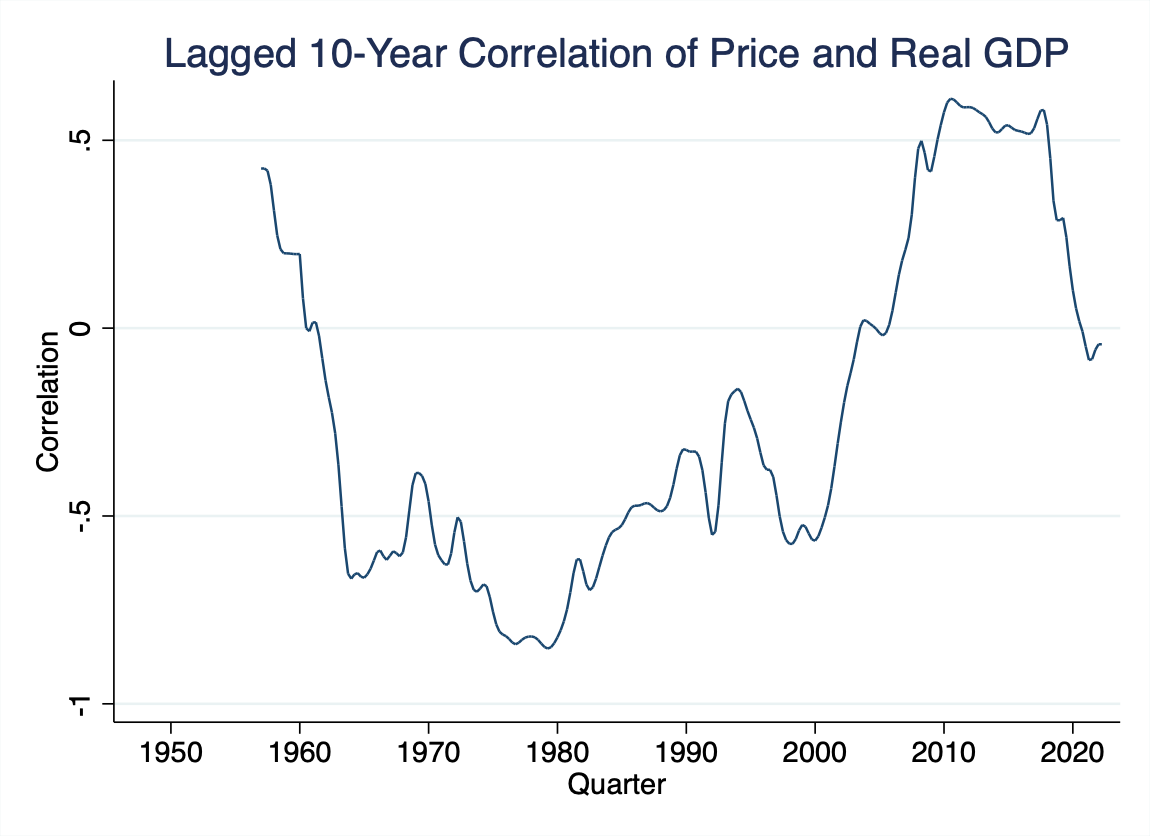
\includegraphics[scale=0.25]{Figures/Fig_13_CycCorrPY.png}
%\end{figure}
%\end{frame}



\begin{frame}
\frametitle[alignment=center]{Implications of Real Business Cycle Theory}
\begin{itemize}
\item In many ways, it seems RBC fits the data well!
\bigskip
\item What are the implications for government policy?
\bigskip
\item Monetary policy should have little stimulative effect
\bigskip
\item Need for stimulus, even during a recession, not good: system is efficient
\bigskip
\item  Most policy comes from fixing distortions--still real distortions that can be fixed
\end{itemize}
\end{frame}

\begin{frame}
\frametitle[alignment=center]{Criticisms of RBC}
\begin{itemize}
\item What is the Solow Residual?  
\bigskip
\item Are productivity drops just mismeasurement of \emph{used} capital?  $$A^{Measured}=\frac{A(K^{True})^\alpha L^{1-\alpha}}{A{K^{Measured}}^\alpha L^{1-\alpha}}=A^{True}\frac{K^{True}}{K^{Measured}}$$
\bigskip
\item So if true, used capital falls, but measured capital doesn't, then measured $A$ will fall
\bigskip
\item Similarly, if we keep workers on payrolls (aka ``labor hoarding," because matching is hard) but true working workers is lower, then what looks like a productivity drop will really be a labor drop
\bigskip
\item Let's go through an example
\end{itemize}
\end{frame}

\begin{frame}
\frametitle[alignment=center]{Labor Hoarding Example}
\begin{itemize}
\item Say that:
$$Y=zK^{0.3}L^{0.7}$$
\item Inititally, $z=1$, $K=100$, and $N=50$, so $Y=61.6$.  
\item Then, a recession hits:  we keep all capital $K=100$, but use only 95\% of it, and labor effort falls by 10\% (even as measured labor stays same)
\item Even though $z$ didn't fall, $K=95$ and $N=45$ (what's actually used) means $Y=56.3$ and:
$$\hat{z}=\frac{56.3}{100^{0.3}50^{0.7}}=0.915$$
\item We measure a 8.5\% drop in TFP even though it didn't drop at all!
\bigskip
\item This difference between what is measured and what is actually used makes cyclicality of TFP a harder concept to hang our hat on!
\end{itemize}
\end{frame}



\begin{frame}
\frametitle[alignment=center]{Keynesian Coordination Failure}
\begin{itemize}
\item So far, no need for government
\bigskip
\item Introduce a ``coordination failure"
\bigskip
\item Your action affects my incentives, mine affects yours (like going to a party)
\bigskip
\item Produce computers $\iff$ produce software
\bigskip
\item Short-run increasing returns in production
\end{itemize}
\end{frame}

\begin{frame}
\frametitle[alignment=center]{Increasing Returns to Scale}
\begin{figure}
\centering
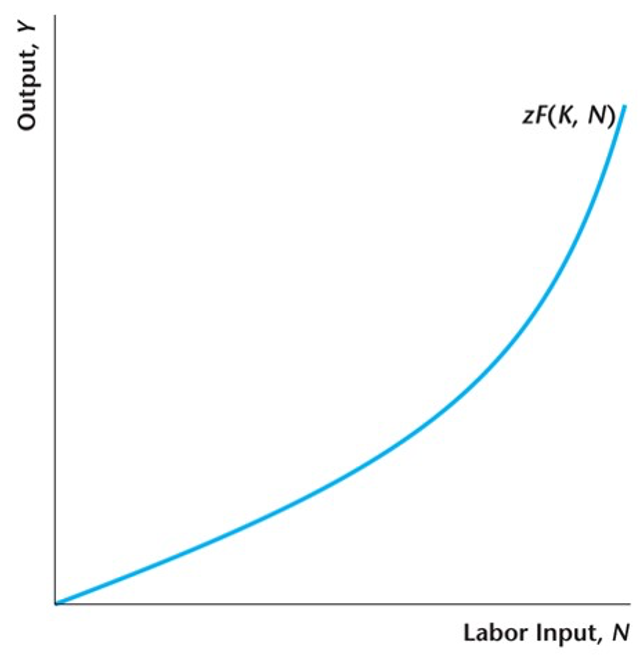
\includegraphics[scale=0.65]{Figures/W_Fig_13pt5.png}
\end{figure}
\end{frame}

\begin{frame}
\frametitle[alignment=center]{Labor Demand is...upward sloping?}
\begin{figure}
\centering
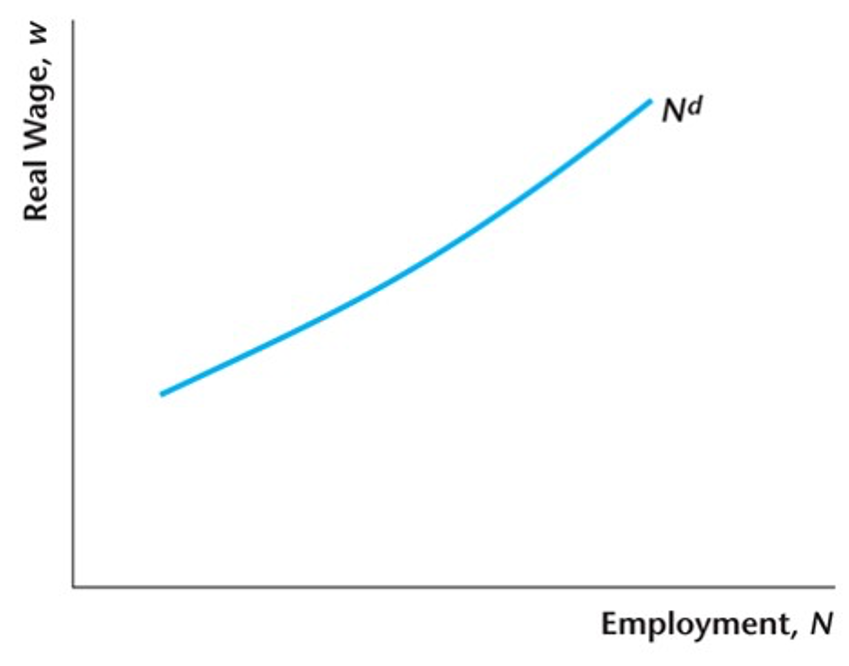
\includegraphics[scale=0.65]{Figures/W_Fig_13pt6.png}
\end{figure}
\end{frame}

\begin{frame}
\frametitle[alignment=center]{Labor demand steeper than labor supply?}
\begin{figure}
\centering
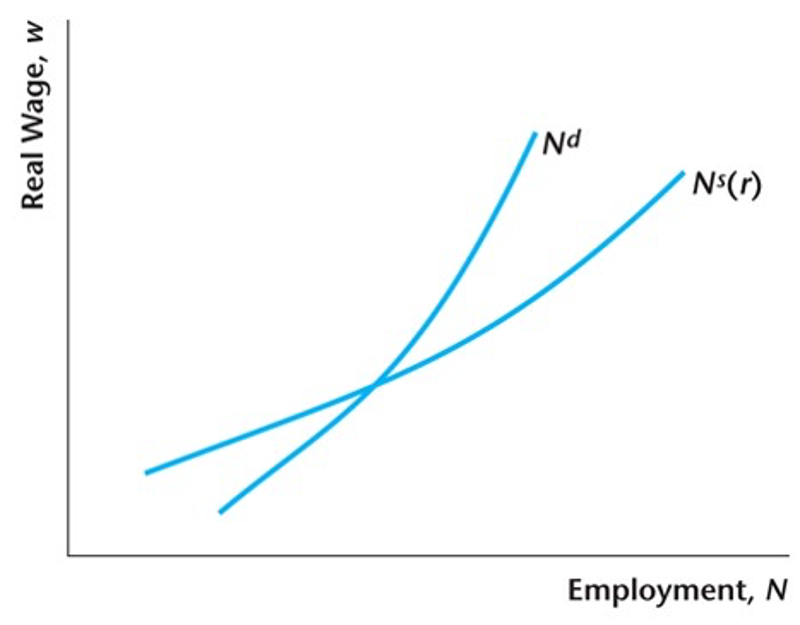
\includegraphics[scale=0.65]{Figures/W_Fig_13pt7.png}
\end{figure}
Things  can be a little upside-down now!
\end{frame}



\begin{frame}
\frametitle[alignment=center]{Supply Curve in Coordination Failure Model}
\begin{figure}
\centering
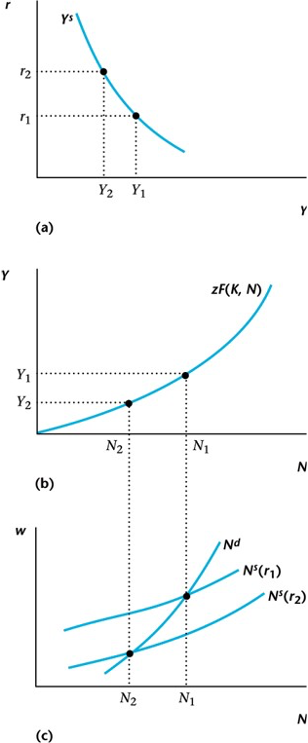
\includegraphics[scale=0.55]{Figures/W_Fig_13pt8.png}
\end{figure}
When interest rate rises now, labor supply increases, \emph{reducing}(!) output (output supply is downward sloping)
\end{frame}

\begin{frame}
\frametitle[alignment=center]{So what's the idea here?}
\begin{itemize}
\item If output supply is downward sloping, we can have it intersect with output demand multiple times (twice, for instance)
\bigskip
\item Two equilibria: 
\begin{enumerate}
\item ``Bad" equilibria: low labor, low production/consumption, higher wages
\bigskip
\item ``Good" equilibria: high labor, high production/consumption, lower wages
\end{enumerate}
\item ``No" reason to be in one vs the other
\end{itemize}
\end{frame}


\begin{frame}
\frametitle[alignment=center]{Coordination Failure Model}
\begin{figure}
\centering
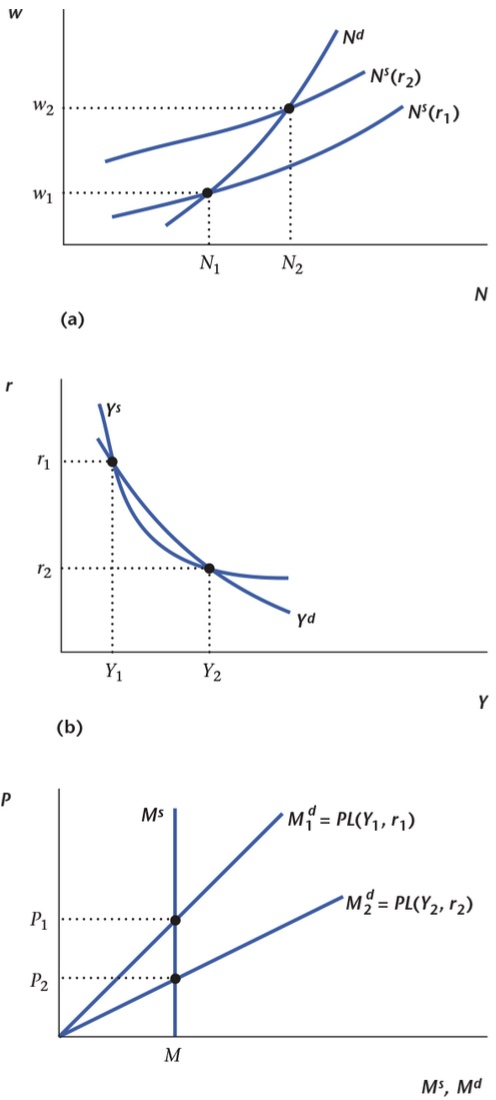
\includegraphics[scale=0.18]{Figures/W_Fig_13pt9.png}
\end{figure}
Because $Y^s$ downward sloping, two equilibrium $Y^*$'s
\end{frame}

\begin{frame}
\frametitle[alignment=center]{Summary of the Coordination Failure Model Predictions}
\begin{table}
\centering
\begin{tabular}{lcc}
\hline\hline
Variable & Data & Model \\
\hline
Consumption & Procyclical & Procylical \\
Investment & Procyclical & Procylical \\
Employment & Procyclical & Procylical \\
Real Wage & Procyclical & Procylical \\
Average Labor Productivity & Procyclical & Procylical \\
\hline\hline
\end{tabular}
\end{table}
Claim:  just like our real business cycle model, which had success in explaining the joint co-movements of variables, coordination failure model has the right set of joint movements!  (A competitior!)
\end{frame}

\begin{frame}
\frametitle[alignment=center]{Money in Coordination Failure}
\begin{itemize}
\item Money is neutral in this model
\bigskip
\item But if everyone \emph{believes} money has an effect, then it would act as a coordiation mechanism
\bigskip
\item Then could get money ``causing" business cycles
\end{itemize}
\end{frame}


\begin{frame}
\frametitle[alignment=center]{Coordination Failure Model}
\begin{figure}
\centering
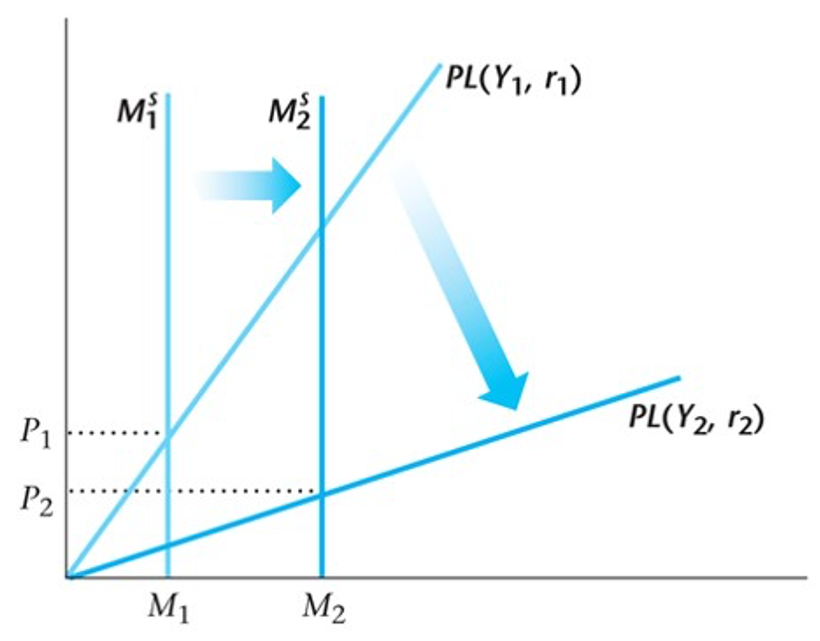
\includegraphics[scale=0.65]{Figures/W_Fig_13pt11.png}
\end{figure}
\end{frame}

\begin{frame}
\frametitle[alignment=center]{Implications of Coordiation Failure Theory}
\begin{itemize}
\item Essentially identical in predictions to RBC
\bigskip
\item However, ``stabilization policy" could have an effect: eliminate two equilibria to be one
\end{itemize}
\end{frame}

\begin{frame}
\frametitle[alignment=center]{Coordination Failure: Smoothing}
\begin{figure}
\centering
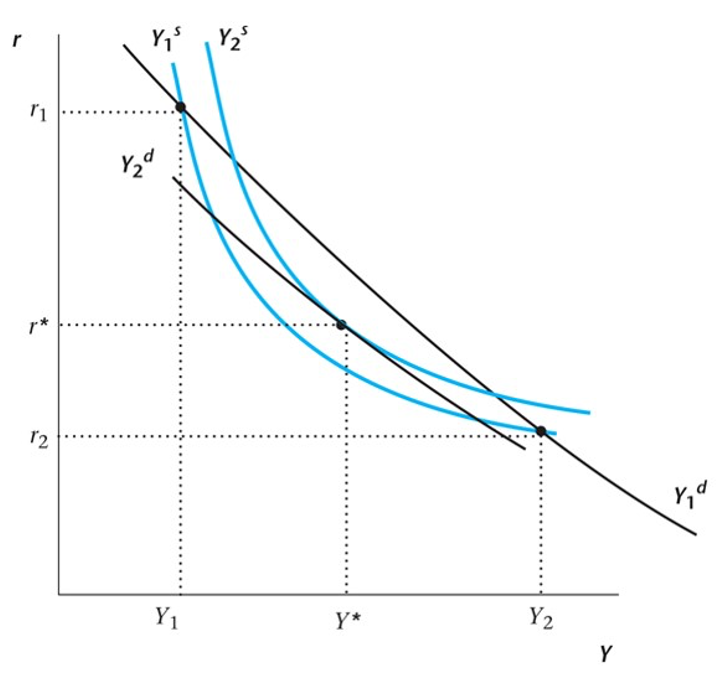
\includegraphics[scale=0.65]{Figures/W_Fig_13pt12.png}
\end{figure}
\end{frame}

\begin{frame}
\frametitle[alignment=center]{Criticisms of Coordination Fialure}
\begin{itemize}
\item Where are the increasing returns?  Hard to find evidence
\end{itemize}
\end{frame}

\begin{frame}
\frametitle[alignment=center]{Business Cycle Theories and the Great Recession}
\begin{itemize}
\item Can our models explain the Great Recession (2008-2009)?
\bigskip
\item First, extract Solow residual (with the caveats we gave above) and compare to GDP
\bigskip
\item Then, see if consumption, investment is consistent with our models
\bigskip
\item Then, see if price level, average productivity, real GDP consistent
\end{itemize}
\end{frame}

\begin{frame}
\frametitle[alignment=center]{Great Recession TFP}
\begin{figure}
\centering
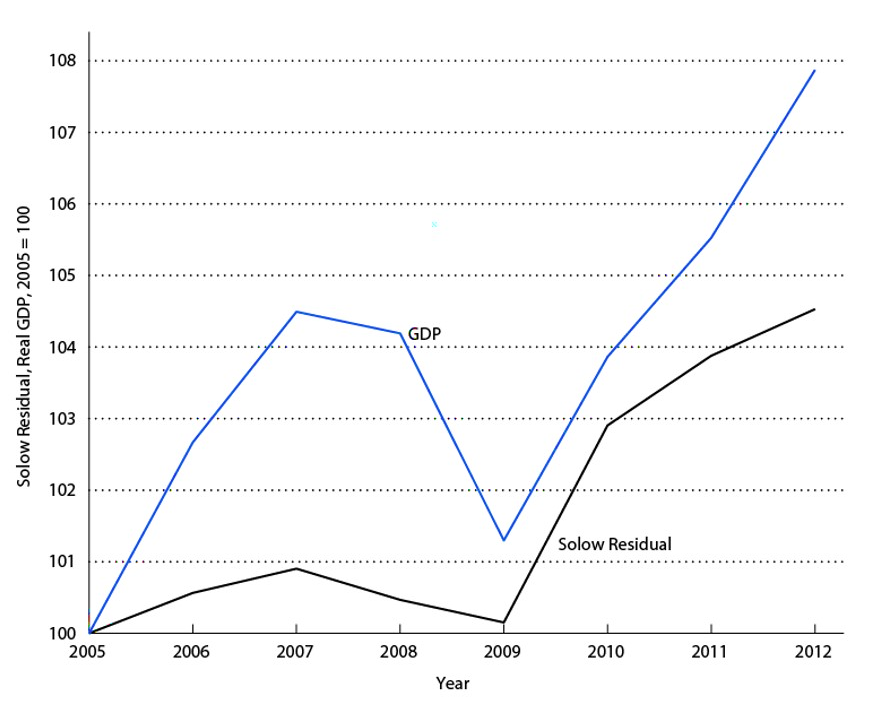
\includegraphics[scale=0.65]{Figures/W_Fig_13pt13.png}
\end{figure}
There is a TFP decline, but it's too small to explain everything
\end{frame}

\begin{frame}
\frametitle[alignment=center]{Great Recession Consumption \& Investment}
\begin{figure}
\centering
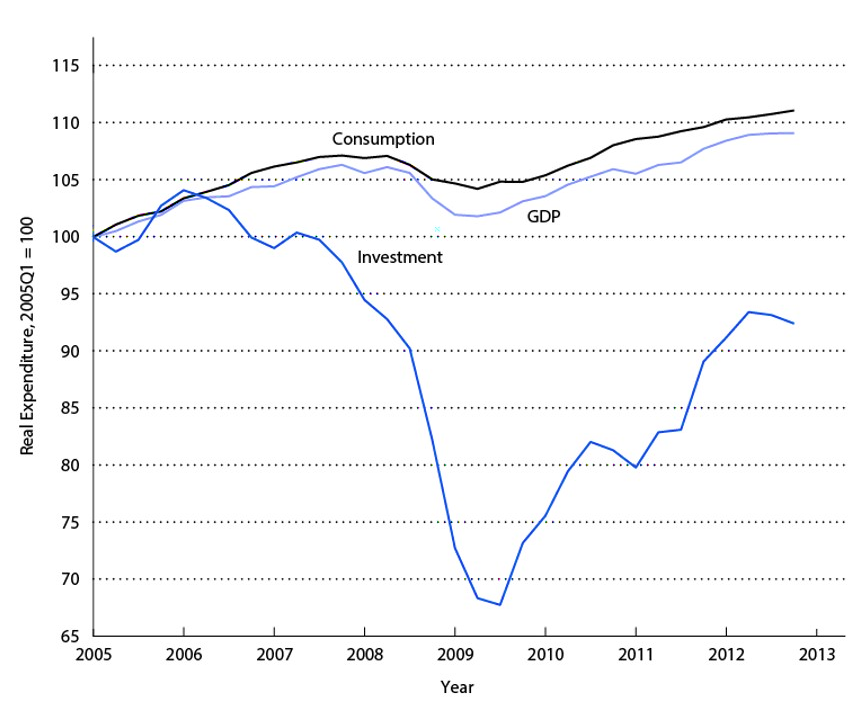
\includegraphics[scale=0.65]{Figures/W_Fig_13pt14.png}
\end{figure}
Consistent with our model (GDP falls, I more volatile, C smoother)
\end{frame}

\begin{frame}
\frametitle[alignment=center]{Great Recession price level and average labor productivity}
\begin{figure}
\centering
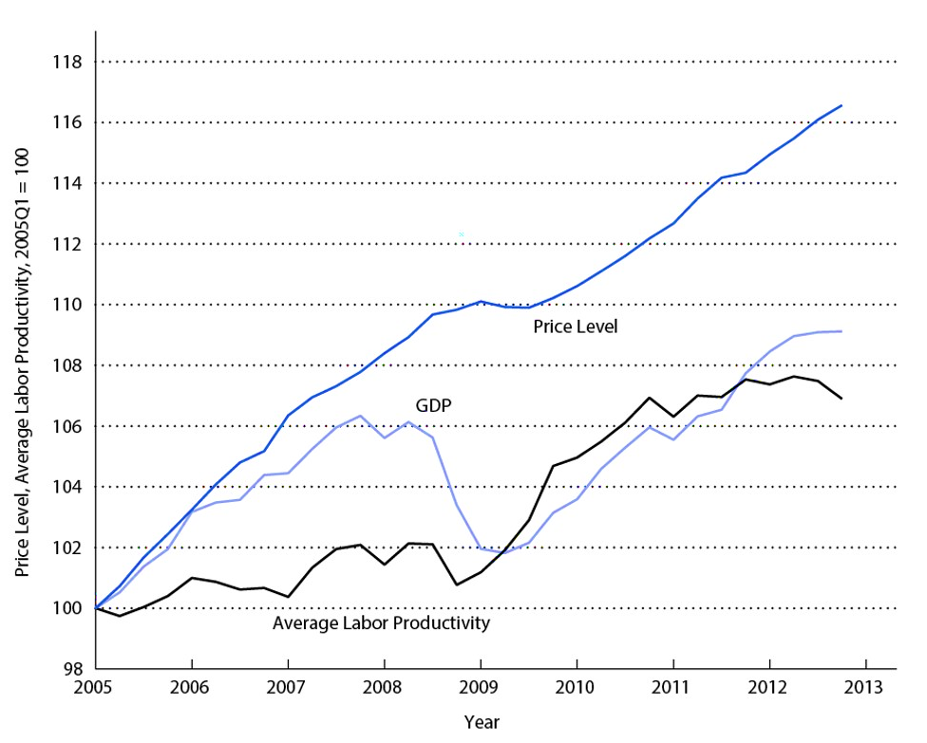
\includegraphics[scale=0.65]{Figures/W_Fig_13pt15.png}
\end{figure}
Price level falls and average labor productivity rose (not consistent with either model)
\end{frame}


\begin{frame}
\frametitle[alignment=center]{Great Recession}
\begin{itemize}
\item Our model is consistent with some of the Great Recession, such as:
\begin{itemize}
\item Some movements in TFP and GDP (but not enough)
\item Qualitative consumption and investment movements
\end{itemize}
\item But doesn't look great on:
\begin{itemize}
\item Fall in price level
\item Qualitative consumption and investment movements
\end{itemize}
\item Work to be done!
\bigskip
\item Next Chapter, we start the New Keynesian model
\end{itemize}
\end{frame}


\end{document}